\documentclass[12pt]{article}

% ---- Mise en page & typographie ----
\usepackage[T1]{fontenc}
\usepackage{amsmath, amssymb}
\usepackage{geometry}
\usepackage{pgfplots}
\usepackage{tikz}
\usepackage{booktabs}
\usepackage{xcolor}
\usepackage{titlesec}
\usepackage{enumitem}
\usepackage{fancyhdr}
\usepackage[hidelinks]{hyperref}
\usepackage{placeins}

\geometry{margin=2.5cm}
\pgfplotsset{compat=1.17}

% ---- Couleurs ----
\definecolor{maincolor}{RGB}{0,90,160}

% ---- Couleur des titres de section (police inchangée) ----
\titleformat{\section}
  {\normalfont\Large\bfseries\color{maincolor}}
  {\thesection}{0.6em}{}
\titleformat{\subsection}
  {\normalfont\large\bfseries\color{maincolor}}
  {\thesubsection}{0.6em}{}

% ---- Pied de page ----
\pagestyle{fancy}
\fancyhf{}
\renewcommand{\headrulewidth}{0pt}
\renewcommand{\footrulewidth}{0pt}
\fancyfoot[C]{\small\thepage}

\begin{document}

% ============================================================
% Page de titre
% ============================================================
\begin{titlepage}
    \centering
    \pagestyle{empty}
    \vspace*{1.5cm}

    {\huge \textbf{Rapport GPGPU}}\\[0.6cm]
    {\Large Implémentation et optimisation de la détection\\ de mouvement d'un flux vidéo}\\[0.5cm]

    \vfill

    {\large \textbf{Auteurs}}\\[0.6cm]
    {\large
    Steeve KE\\[0.15cm]
    Clément GRÉGOIRE\\[0.15cm]
    Marcel PECQUEUX\\[0.15cm]
    Ivan HUARD
    }

    \vfill

    {\large \today}

    \vspace*{1cm}
\end{titlepage}

\newpage
\tableofcontents
\newpage

%============================================================
\section{Description du sujet : Pipeline en 4 phases principales}

\subsection{Calcul de différence avec la frame précédente}
Le sujet propose de renvoyer directement la couleur du réservoir de poids maximal comme estimation du fond, puis de soustraire ce fond de la frame courante pour obtenir le masque de mouvement. Dans notre implémentation, on s'écarte de cette approche : le fond n'étant pas unimodal (reflets, léger bruit de caméra, etc.), se baser uniquement sur le réservoir dominant provoquait de nombreux faux positifs dès qu'un pixel de fond variait légèrement. On calcule donc à la place, dans la même passe, la distance minimale entre le pixel courant et l'ensemble des réservoirs suffisamment établis, ce qui capture mieux la nature multi-modale du modèle. Le fallback sur le réservoir de poids max (comportement du sujet) n'est utilisé que tant qu'aucun réservoir n'est encore assez établi.
\subsection{Suppression du bruit par ouverture morphologique}
L'ouverture est une érosion suivie d'une dilatation appliquée sur le masque de différence. L'érosion remplace chaque pixel par le minimum de ses voisins dans un rayon donné (RADIUS), ce qui élimine les petits points isolés (bruit) mais rétrécit aussi les vraies formes détectées. La dilatation fait l'inverse (maximum des voisins) et restaure la taille des objets qui ont survécu à l'érosion.

\subsection{Seuillage d'hystérésis}

\subsection{Masquage final}

\subsection{Ce qui a été implémenté sur GPU}
On a fait le choix d'implémenter toute la pipeline (les 4 étapes) sur GPU pour minimiser le transfert de mémoire CPU $\leftrightarrow$ GPU.

\bigskip

%============================================================
\section{Répartition des tâches par membre du groupe}

\subsection{Baseline}
\begin{itemize}[leftmargin=1.5cm]
    \item Différence + ouverture \hfill --- \textbf{Ivan}
    \item Seuillage d'hystérésis \hfill --- \textbf{Steeve}
    \item Masquage \hfill --- \textbf{Marcel}
\end{itemize}

\subsection{Portage GPU}
\begin{itemize}[leftmargin=1.5cm]
    \item Ouverture (kernel érosion + dilatation) \hfill --- \textbf{Marcel}
    \item Fonction différence \hfill --- \textbf{Clément}
    \item Seuillage d'hystérésis \hfill --- \textbf{Ivan + Steeve}
    \item Masquage \hfill --- \textbf{Marcel}
\end{itemize}

\subsection{Optimisations GPU}
\begin{itemize}[leftmargin=1.5cm]
    \item Optimisation mémoire + AoS to SoA \hfill --- \textbf{Ivan}
    \item Optimisation alignement mémoire (\texttt{mallocPitch} + \texttt{alignas}) \hfill --- \textbf{Steeve}
    \item \textit{... à compléter}
\end{itemize}

\bigskip

%============================================================
\section{Benchmarks et graphiques des performances des versions (CPU + GPU + GPU Optimisé)}
\subsection{Protocole du benchmark}
\subsection*{Protocole de test}
\begin{itemize}[leftmargin=1.5cm]
    \item \textbf{Vidéo(s) utilisée(s)} : Pour l'ensemble des tests qui suivent la vidéo "video03.avi" fourni par le sujet (résolution de 320 × 240, 60 frames/secondes pour une vidéo de 28 secondes, vidéo d'une autoroute avec des voitures qui passent au fur et à mesure que la vidéo défile)
    \item \textbf{Configuration matérielle} : CPU \textit{Intel(R) Core(TM) i5-11400H @ 2.70GHz}, GPU \textit{RTX 3050Ti laptop}, driver CUDA \textit{version 12.8}
    \item \textbf{Méthode de mesure} : La vidéo fait 28 secondes, à 60 FPS, on a $\# FPS = 60*28/(tot)$ avec tot le nombre de secondes total. Le même principe est utilisé pour le temps moyen par frame (en millisecondes).
    \item \textbf{Métrique} : temps moyen par frame (ms) et FPS équivalent
\end{itemize}
 
\bigskip
 
\subsection{V0 baseline}
Temps total : 1minute 37secondes \newline
Temps moyen par frame : 58ms \newline
FPS : 17 \newline

\subsection{V1.0.0 GPU non-optimisé}
Temps total : 2secondes24 \newline
Temps moyen par frame : 1,337ms \newline
FPS : 747,9 fps \newline
 
\subsection{V1.0.1 GPU accès mémoire \& transfert de données optimisés}
Temps total : 2secondes06 \newline
Temps moyen par frame : 1,231ms \newline
FPS : 812,6 fps \newline
 
\subsection{V1.0.2 GPU ...}
Temps moyen par frame : xx \newline
FPS : XX \newline
 
\bigskip
 
\subsection{Synthèse comparative des versions}
 
Le tableau~\ref{tab:synthese} et la figure~\ref{fig:speedup} résument les performances de l'ensemble des versions et l'apport de chaque optimisation par rapport à la baseline CPU.
 
\begin{table}[h!]
    \centering
    \begin{tabular}{lccc}
        \toprule
        \textbf{Version} & \textbf{Temps moyen / frame (ms)} & \textbf{FPS} & \textbf{Speedup vs V0} \\
        \midrule
        V0 (baseline CPU)                          & \textit{58} & \textit{17} & $\times 1.0$ \\
        V1.0.0 (GPU non-optimisé)                  & \textit{1337} & \textit{747,9} & \textit{...} \\
        V1.0.1 (accès mémoire \& transfert)         & \textit{1231} & \textit{812,6} & \textit{...} \\
        V1.0.2 (\textit{...})                       & \textit{...} & \textit{...} & \textit{...} \\
        \bottomrule
    \end{tabular}
    \caption{Comparaison des performances par version}
    \label{tab:synthese}
\end{table}

 


%============================================================
\section{Analyse des performances et des bottlenecks (graphiques Nsight / nvprof)}
\label{sec:nsight-bottlenecks}
 
\subsection{Premier bottleneck mémoire}
Le premier bottleneck auquel nous avons fait face est non pas causé par un kernel mais par la gestion de la mémoire entre les kernels. Il nous fallait donc commencer par optimiser les tranfert mémoire avant de s'attaquer aux kernels, qui, proportionnellement, étaient moins gourmands en ressources. Après analyse de notre code, au lieu de définir un seul buffer que nous aurions réutilisé tout au long des kernels, nous faisions des tranfert mémoire inutile Device vers Host puis Host vers Device entre les différents kernels.
\newline
\begin{figure}[htbp]
    \centering
    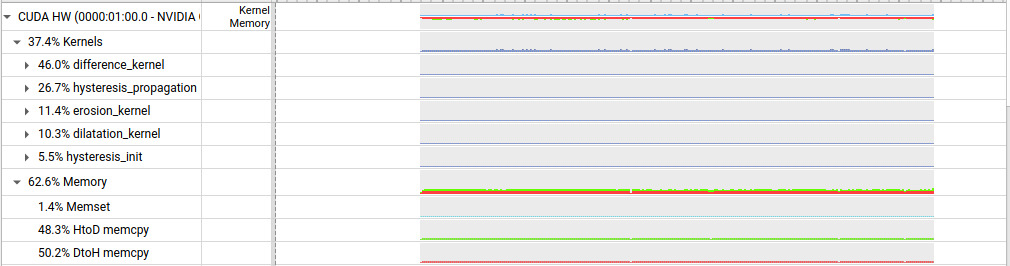
\includegraphics[width=0.85\linewidth]{nsightSYSnoOpti.jpg}
    \caption{First NSight System capture (V1.0.0)}
    \label{fig:sys-v100}
\end{figure}
\FloatBarrier

\subsection{Optimisation de transfert mémoire}
En gardant le même buffer tout au long des kernels (sans transfert inutiles) nous obtenons une meilleure répartition de travail entre mémoire et kernels. \newline
\begin{figure}[htbp]
    \centering
    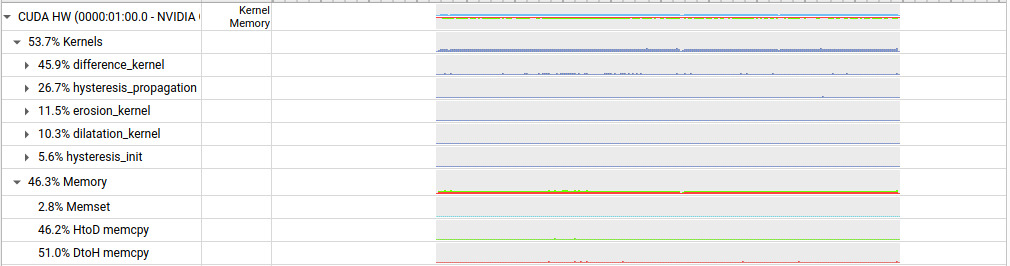
\includegraphics[width=0.85\linewidth]{nsightSYSoptiMem.jpg}
    \caption{NSight System after memory optimization}
    \label{fig:sys-optimem}
\end{figure}
\FloatBarrier

\subsection{SoA vers AoS}
D'après la figure 3 de nsight système, c'est désormais les kernels qu'il faut optimiser. En regardant la liste que nous fait le profiling, on voit que le kernel le plus gros en pourcentage est \texttt{difference\_kernel}. D'après les informations récoltés par NSight Compute sur ce même kernel, le problème vient d'un accès mémoire non-coalescent.
\newline
Uncoalesced AoS: \newline
\begin{figure}[htbp]
    \centering
    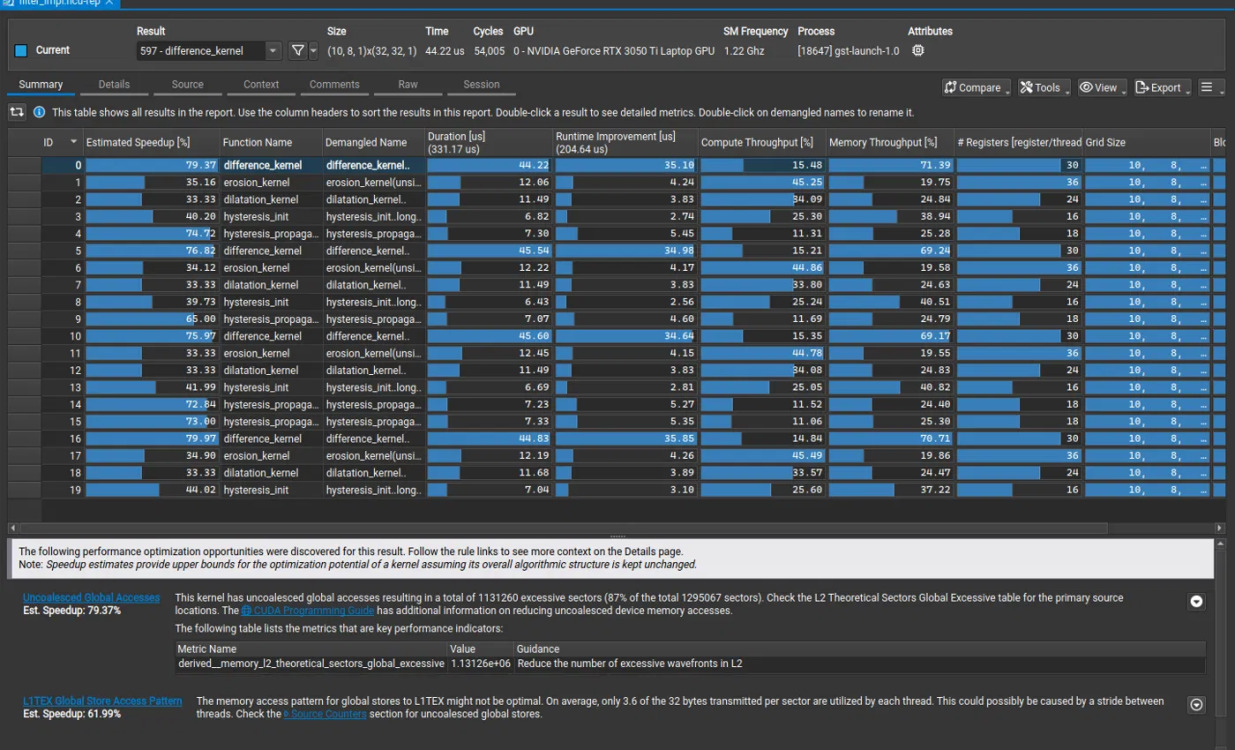
\includegraphics[width=0.85\linewidth]{nsightcuBeforeCoalesced.jpg}
    \caption{NSight Compute before AoS optimization}
    \label{fig:cu-aos-before}
\end{figure}
\FloatBarrier
Dans l'étape (1) de différence, les réservoirs sont stockés de manière AoS, c'est à dire qu'on a une liste de structure, chaque structure contenant un bytes par canal + un entier pour stocker le poids de la couleur, c'est la raison pour laquelle les threads effectuent un accès non-coalescent, quand deux threads veulent accéder (simultanément) à leur premier réservoir, ils doivent charger chacun une partie de la mémoire très éloignée chaque pixel ayant ses réservoirs les uns à la suite des autres.
Pour régler ce problème, on ré-organise la structure de remplissage (sans changer la taille du tableau) pour mettre les premiers réservoir de chaque pixels les uns à la suite des autre et suivre un pattern SoA. De cette manière, quand nos threads accéderont simultanément à leurs premier réservoir respectif, un seul (ou peu) appel de retrait mémoire sera suffisant (chaque appel mémoire impliquant également l'appel ses voisins les plus proches).
\newline
Coalescent access with SoA : \newline
\begin{figure}[htbp]
    \centering
    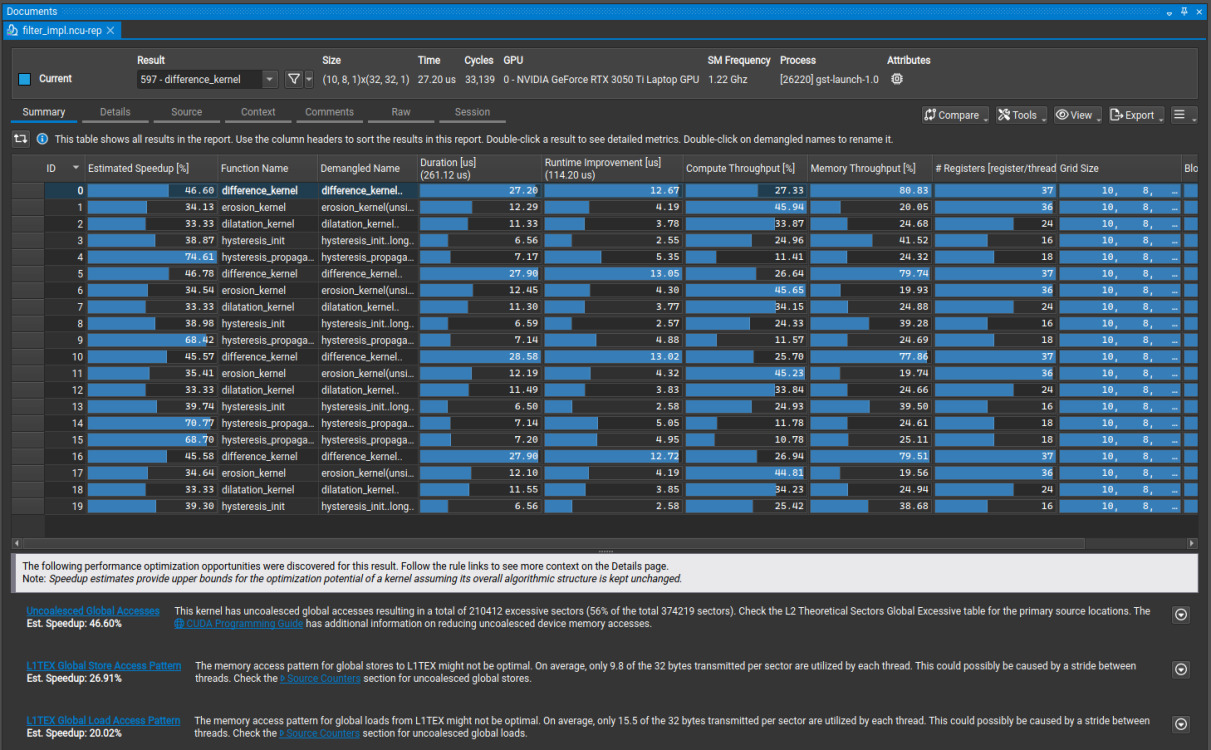
\includegraphics[width=0.85\linewidth]{nsightcuAfterCoalesced.jpg}
    \caption{NSight Compute after AoS optimization to SoA}
    \label{fig:cu-aos-after}
\end{figure}
\FloatBarrier
Après cet optimisation un speedup à bien eu lieu, et, logiquement, nous avons aussi une diminution de \texttt{estimated speedup} de NSight Compute.

\bigskip

%------------------------------------------------------------
\end{document}